\documentclass[10pt]{article}

% Lines beginning with the percent sign are comments
% This file has been commented to help you understand more about LaTeX

% DO NOT EDIT THE LINES BETWEEN THE TWO LONG HORIZONTAL LINES

%---------------------------------------------------------------------------------------------------------

% Packages add extra functionality.
\usepackage{
	times,
	graphicx,
	epstopdf,
	fancyhdr,
	amsfonts,
	amsthm,
	amsmath,
	algorithm,
	algorithmic,
	xspace,
	hyperref}
\usepackage[left=1in,top=1in,right=1in,bottom=1in]{geometry}
\usepackage{sect sty}	%For centering section headings
\usepackage{enumerate}	%Allows more labeling options for enumerate environments 
\usepackage{epsfig}
\usepackage[space]{grffile}
\usepackage{booktabs}
\usepackage{amsmath}
\usepackage[super]{nth}
\usepackage{array}

% This will set LaTeX to look for figures in the same directory as the .tex file
\graphicspath{.} % The dot means current directory.

\pagestyle{fancy}

\lhead{\YOURID}
\chead{\MyLang: Language Specification}
\rhead{\today}
\lfoot{CSCI 334: Principles of Programming Languages}
\cfoot{\thepage}
\rfoot{Spring 2022}

% Some commands for changing header and footer format
\renewcommand{\headrulewidth}{0.4pt}
\renewcommand{\headwidth}{\textwidth}
\renewcommand{\footrulewidth}{0.4pt}

% These let you use common environments
\newtheorem{claim}{Claim}
\newtheorem{definition}{Definition}
\newtheorem{theorem}{Theorem}
\newtheorem{lemma}{Lemma}
\newtheorem{observation}{Observation}
\newtheorem{question}{Question}

\setlength{\parindent}{0cm}
%---------------------------------------------------------------------------------------------------------

% DON'T CHANGE ANYTHING ABOVE HERE

% Edit below as instructed
\usepackage{adjustbox}
\newcommand{\MyLang}{PixelPunk}	% Replace MyLang with your language name #
\newcommand{\PartnerOne}{Max Kan}	% Replace PartnerOne with your name #
\newcommand{\PartnerTwo}{Rijul Jain}	% Replace PartnerTwo with your partner's name #
\newcommand{\YOURID}{\PartnerOne{} + \PartnerTwo{}} % Remove \PartnerTwo if working alone.


\title{\MyLang: Language Specification}
\date{Spring 2022}
\author{\PartnerOne{} and \PartnerTwo{}} % Remove \PartnerTwo if working alone.

\begin{document}
\maketitle

\vspace{\baselineskip}	% Add some vertical space

% Refer to the lab handouts to determine what should go in each of these sections.  Each lab is additive.  So lab 8 should include everything you wrote in lab 7.  Lab 9 should include everything you wrote in lab 8, etc.

\section{Introduction}
    Collins Dictionary's word of the year for 2021, NFTs (non-fungible tokens) have recently exploded in popularity. Often compared to fine art collecting, NFTs come in many different shapes and forms, but one particular style of NFT art has come to define the space: profile pictures. If you've ever seen some tech celebrity or crypto billionaire with a strange looking monkey or pixelated profile picture on Twitter, chances are, it was an NFT. \\
    
    With this trend in mind, our goal is to create a programming language that allows non-technical users to easily create custom profile picture art. Using the popular "CryptoPunks" collection of NFTs as inspiration, we hope to foster creativity and inspire more people to check out both the NFT and programming language spaces. At the same time, this programming language is also a social commentary on the absurdity of NFTs; if we can make it laughably easy for anyone to make CryptoPunk-style NFTs with the PixelPunk programming language, we are able to highlight the confusing question of why these things sell for so much money when they're able to be made and imitated so easily. 
		
\section{Design Principles}

    We want to create an intuitive, elegant language that allows for simple programs to result in extremely creative profile picture pixel art. Our data types in this language use familiar terms that are obviously sensible parts of a profile picture, like Head, Background, Eyes, and Hat, to make things transparent for the inexperienced user.
    
    Since the output is a pixel art profile picture that is 24x24 pixels, the user can immediately see the results of their programs. This makes learning to program in PixelPunk very easy, and makes trial and error experimentation for creating wild pixel art even more accessible and approachable. 

\section{Example Programs}

\begin{enumerate}
\item 
\begin{verbatim}
    // This program exhibits that the two required attributes are a head
    // and a background. Others are optional.
    
    Head head = {shape=oval, color=blue, size=large}
    Background background = {color=white}
    
    PixelPunk p = {head, background}
    
    // Outputs a 24x24 pixel art profile picture 
    p.output()
\end{verbatim}
\item
\begin{verbatim}
    // This program uses both the two required and some optional
    // pre-defined attributes.
    
    // It will aim to look like Steve Jobs.
    
    Head head = {shape=oval, color=skin1, size=medium}
    Background background = {color=white} 
    
    // The following are optional and pre-defined
    Eyes eyes = {color=brown, glasses=round, size=medium}
    Hair hair = {style=bald}
    FacialHair facialHair = {style=beard, color=gray}
    Clothes clothes = {style=turtleneck, color=black}
    
    PixelPunk p = {head, background, eyes, hair, facialHair, clothes}
    
    // Outputs a 24x24 Steve Jobs-esque pixel art profile picture 
    p.output()
    
\end{verbatim}
\item
\begin{verbatim}
    // This program now incorporates user-defined attributes
    
    
    Head head = {shape=oval, color=skin1, size=medium}
    Background background = {color=white} 
    
    Attribute helmet = {
        Pixel(row=[5,10], col=[3,8], color="#FFD700")
        Pixel(row=[7,10], col=[5,8], color=black)
        }
    
    
    PixelPunk p = {head, background, helmet}
    
    // Outputs a 24x24 custom Daft Punk-esque pixel art profile picture 
    p.output()
    
\end{verbatim}
\end{enumerate}

\section{Language Concepts}

    Every profile picture, which is invariably what PixelPunk programs will output, is a 24x24 grid of pixels. The very base primitives this language relies on are int and string. The most basic combining form is a Pixel, which consists of int row, int col, and string color. Pixels are used to create another combining form, Attribute, which is a collection of Pixels to create recognizable features like Head, Background, Eyes, and Nose. There are pre-defined Attributes with pre-defined parameters, and the user has the power to create custom Attributes and define their own parameters at their discretion. 

\section{Syntax}

    The overall result of a program will be a 24x24 grid of Pixels.
    Each Pixel has a row, column, and color property. The user can modify particular Pixels by changing their inputs for these parameters. 
    The grid also consists of Attributes, which are made up of Pixels. There are pre-defined Attributes, two of which (Head and Background) are required for any PixelPunk program. The user can incorporate more pre-defined Attributes, like Eyes and Nose, or create their own custom Attributes by specifying the Pixel range they want to modify and how. 
    
    This will result in a square pixel art profile picture of 576 pixels total. \\
    
   Below is a minimal formal grammar for the PixelPunk language.
   \begin{verbatim}
   <PixelPunk> ::= <Attribute>+
   <Attribute> ::= <Pixel>+
   <Pixel> ::= <row><col><Color>
   <Color> ::= #<hex><hex><hex><hex><hex><hex>
   <hex> ::= 0 | 1 | 2 | 3 | 4 | 5 | 6 | 7 | 8 | 9 | A | B | C | D | E | F
   <row> ::= 0 | 1 | 2 | 3 | 4 | 5 | 6 | 7 | 8 | 9 | 10 | 11 | 12 | 13 | 14 
   		| 15 | 16 | 17 | 18 | 19 | 20 | 21 | 22 | 23 | 24
   <col> ::= 0 | 1 | 2 | 3 | 4 | 5 | 6 | 7 | 8 | 9 | 10 | 11 | 12 | 13 | 14 
   		| 15 | 16 | 17 | 18 | 19 | 20 | 21 | 22 | 23 | 24
   \end{verbatim}
    
    

\section{Semantics}
    \begin{enumerate}
    \item 
    The primitive kinds of values are technically int and string, but for the user, the most basic building block is the Pixel. The ints are used for specifying the row and col of the pixel, and the string is used to specify the color.
    
    \item
    The compositional elements are Attributes, which are a composite of Pixel(s). They can be pre-defined, like the Attribute Head, that has pre-defined parameters for the user to optionally work with, such as size and color. All of our parameters are essentially functions that modify Pixels. They can also be custom-defined by the user, in which case, the user hard codes the Pixel placements.
    
    \item
    Here is a table of minimal semantics for the PixelPunk language. \\
	\begin{table}[h]
	\begin{adjustbox}{width=\columnwidth,center}
	\begin{tabular}{lllll}
	\hline
	Syntax                                     & Abstract Syntax            & Type              & Prec./Assoc. & Meaning                                                                                                                                                                  \\ \hline
	x                                          & row of int                 & int               & n/a          & x is a primitive, represented by F\# Int32 type.                                                                                                                         \\
	y                                          & col of int                 & int               & n/a          & y is a primitive, represented by F\# Int32 type.                                                                                                                         \\
	"c"                                        & hex of string              & string            & n/a          & c is a primitive hex digit represented by the F\# string type                                                                                                            \\
	"\#cccccc"                                 & Color of string            & string            & 1/left       & Color is six hex digits put together as an F\# string to represent a hex color code.                                                                                     \\
	(x, y, "\#cccccc")                         & Pixel of int * int * Color & int * int * Color & 2/left       & Pixel contains int row, int col, and a Color as a three-tuple.       \\
	{[}(x, y, "\#cccccc"); ... {]}             & Attribute of Pixel+        & Pixel list        & 3/left       & Attribute is simply an F\# list of Pixels; it serves as a combining form to create any grouping of Pixels.                                                               \\
	{[}{[}(x,y, "\#cccccc"); ... {]} ; ... {]} & PixelPunk of Attribute+    & Attribute list    & 4/left       & The ultimate PixelPunk is a list of all the Attributes that comprise the final image.
	\end{tabular}
	\end{adjustbox}
	\end{table}
	
    \item 
    The program is representable by an AST that consists of the PixelPunk grid at the top, branching into two or more Attributes, which branch into one or more Pixels. Simple and elegant. The rough hierarchy sketch is shown below.
    \begin{center}
    	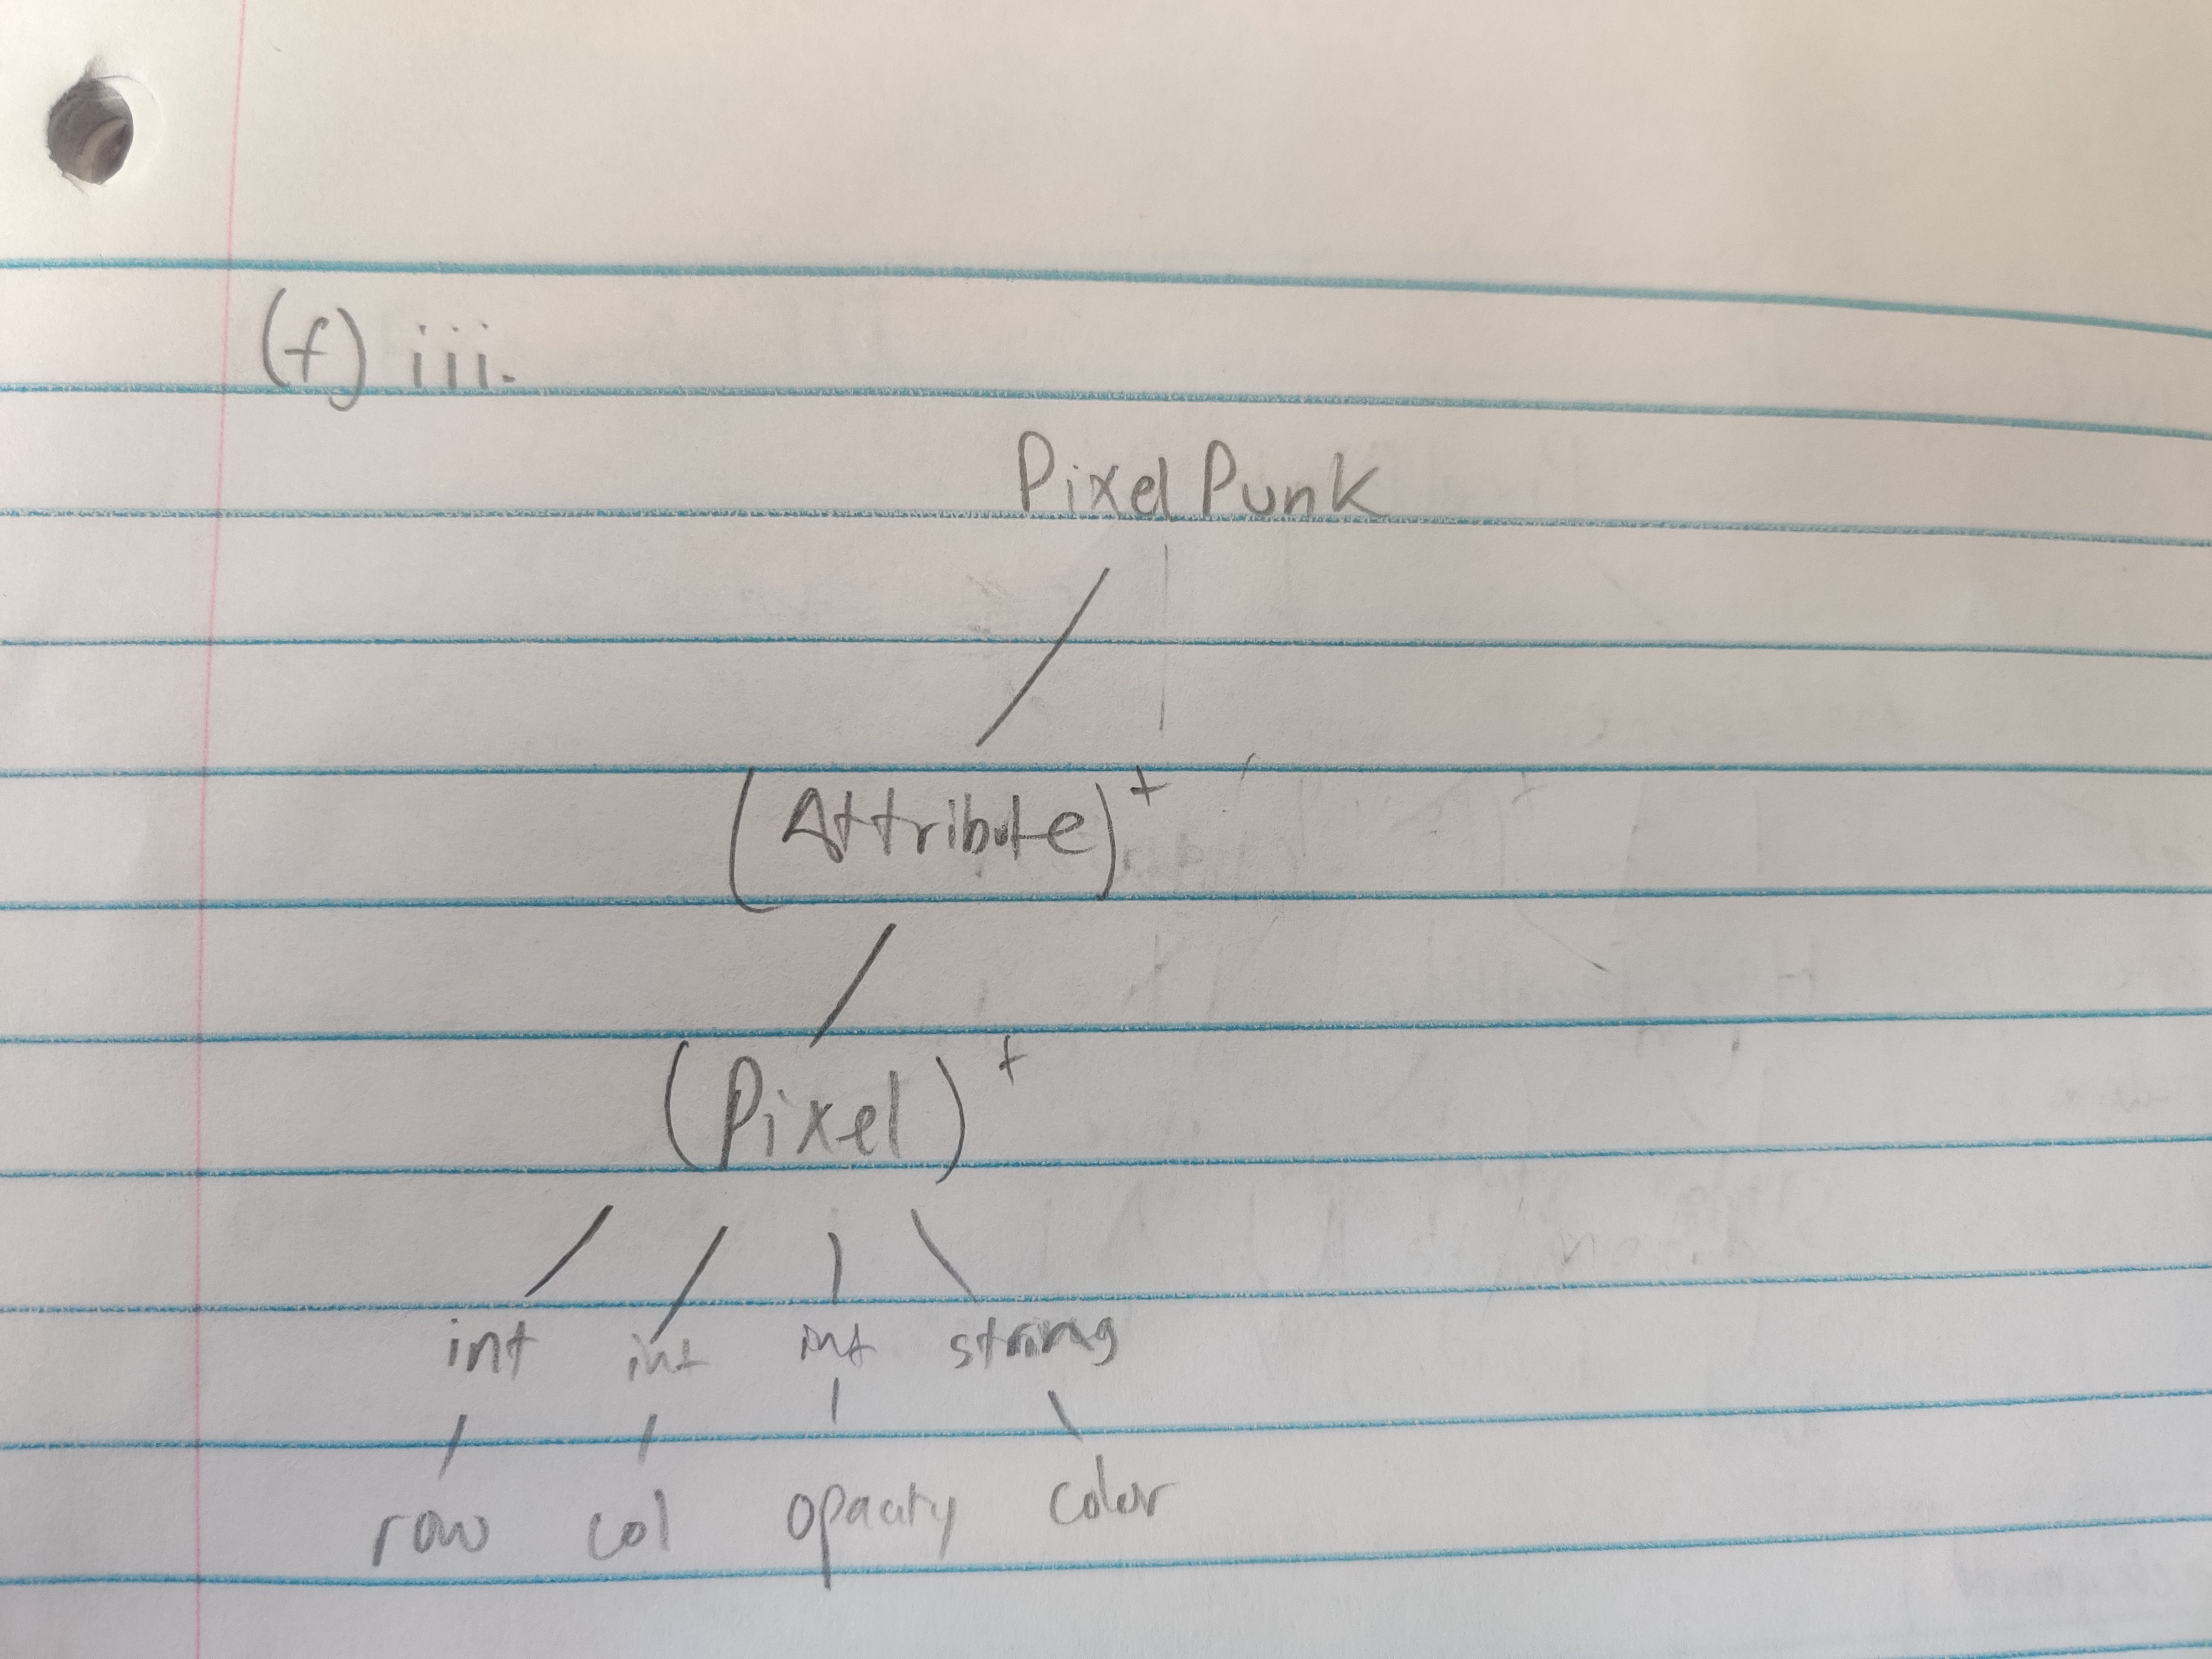
\includegraphics[width=0.75\textwidth]{images/f.jpg}
    \end{center}
    
    \item To reiterate, pixels have a row, column, and color specifier. Everything else is just made of pixels. Below are the three ASTs for the three example programs.
    \begin{center}
    	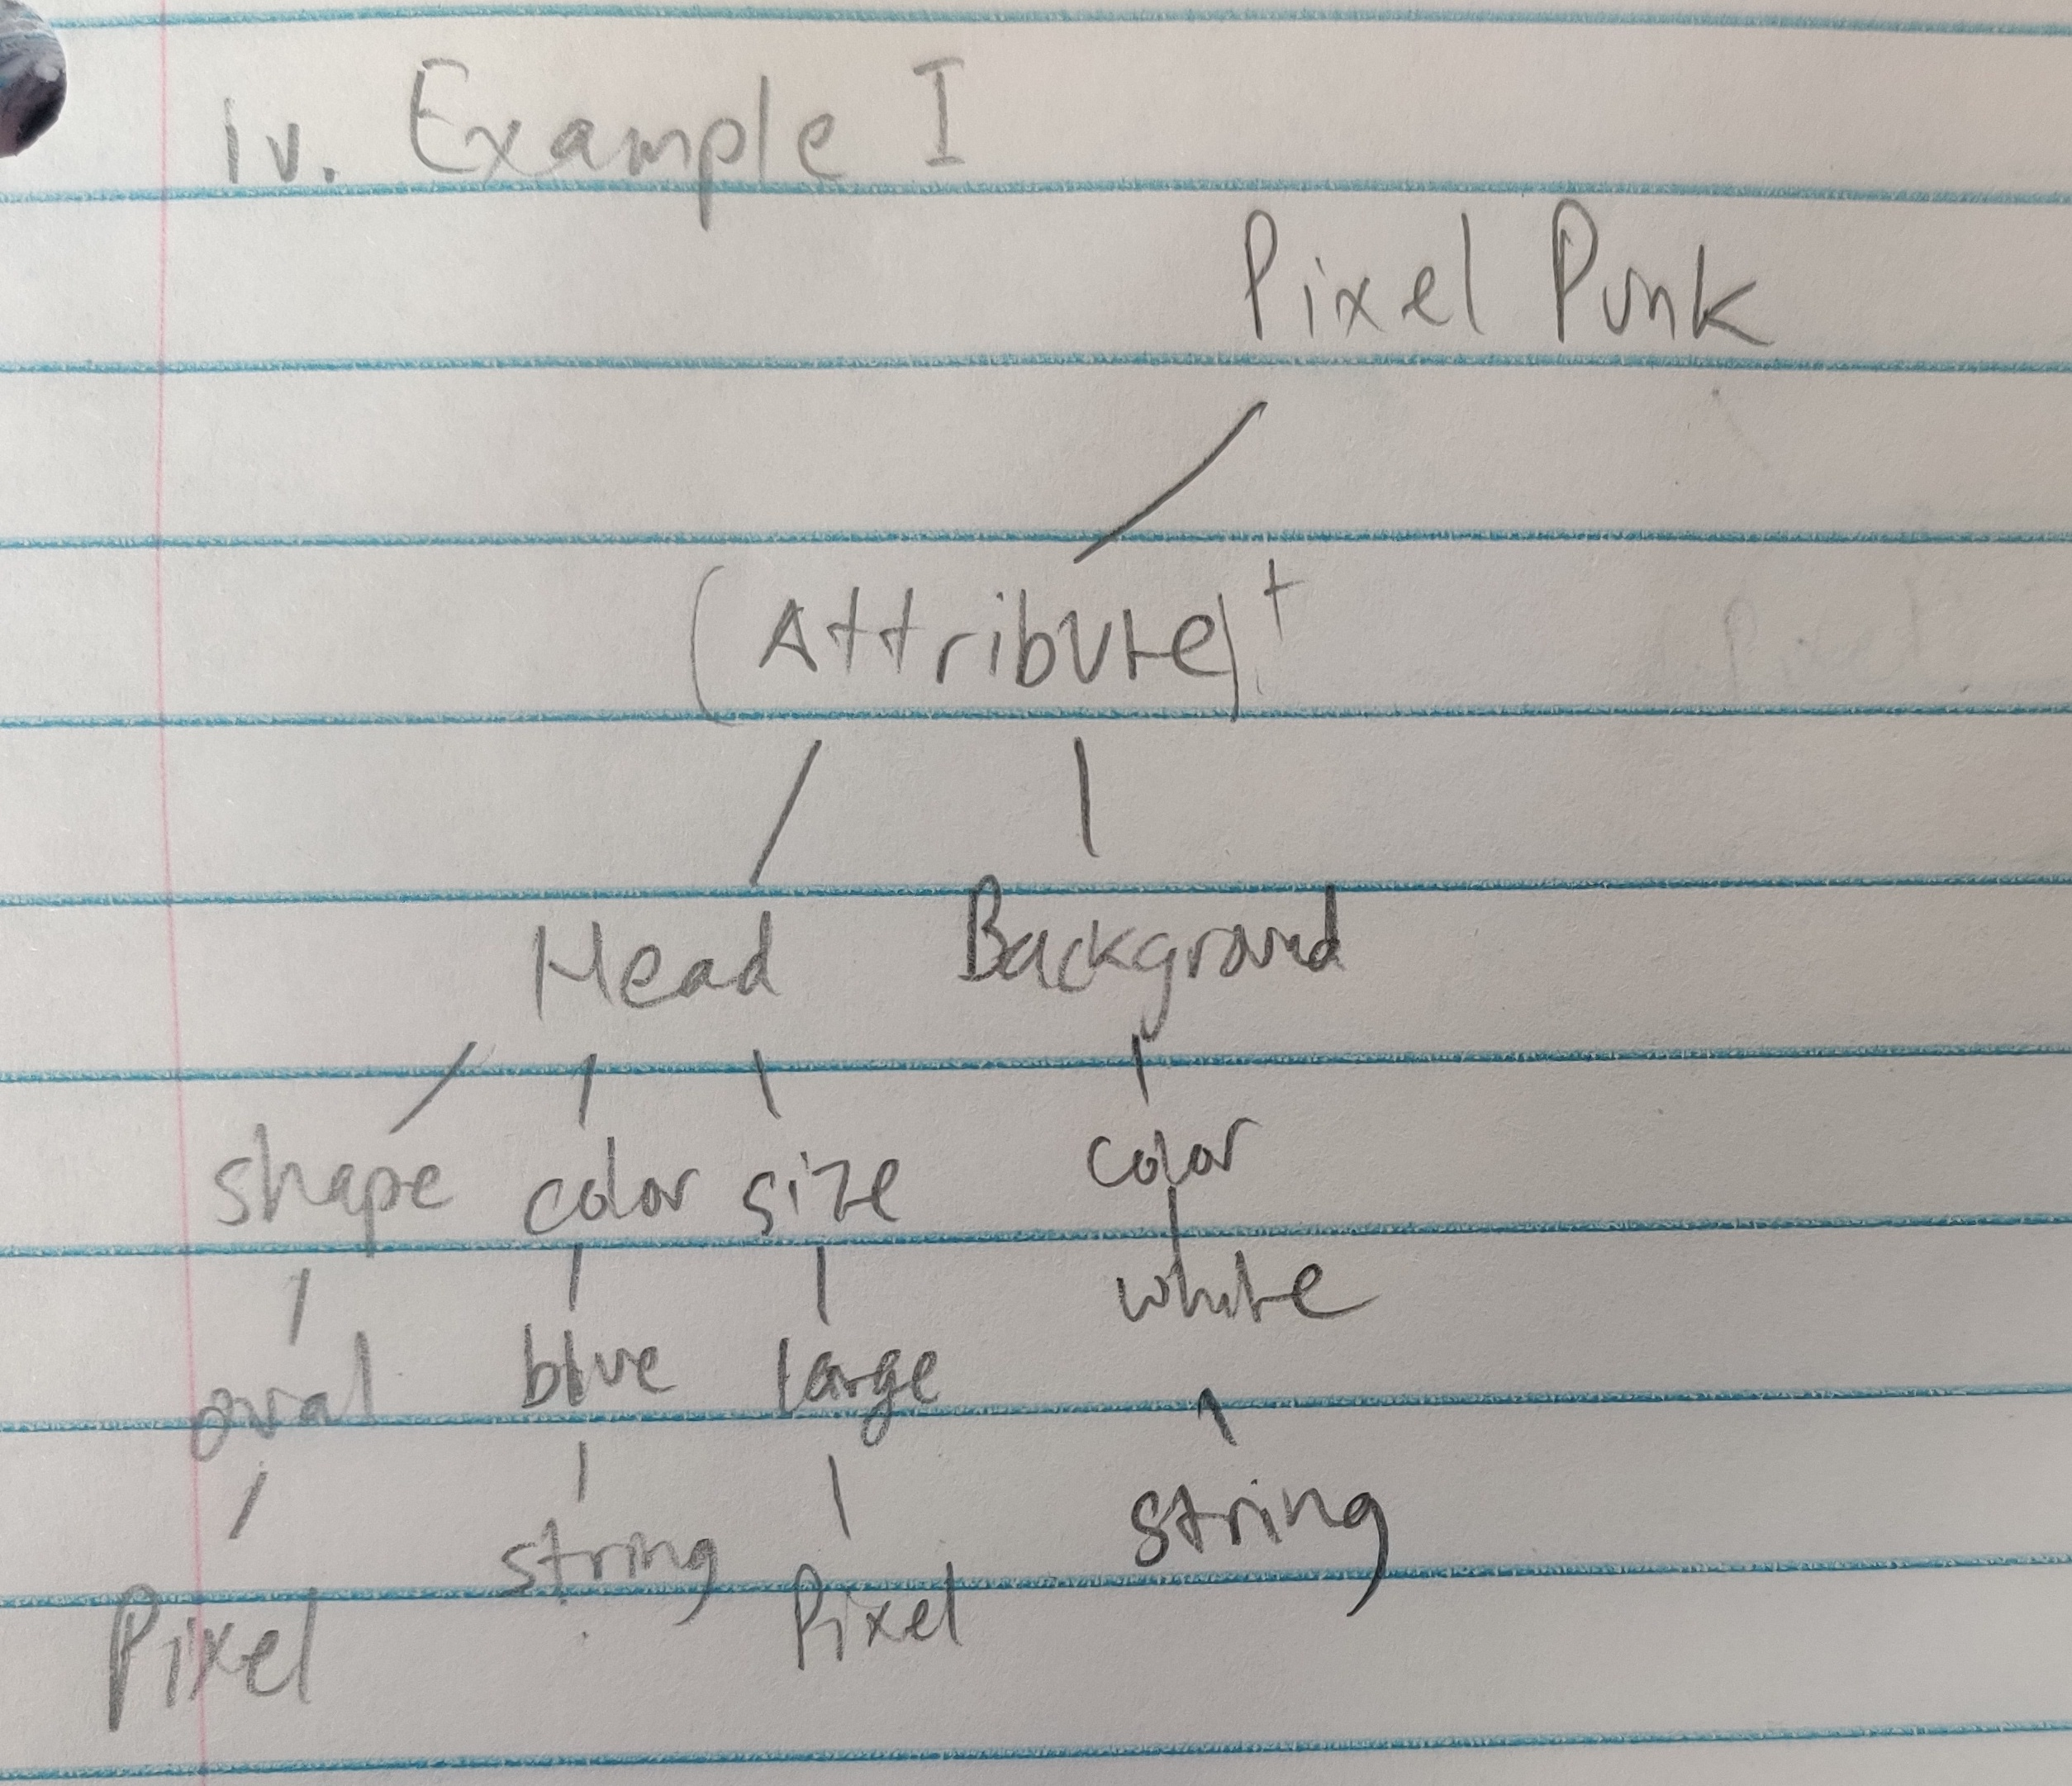
\includegraphics[width=0.75\textwidth]{images/example1.jpg}
    \end{center}
    \begin{center}
    	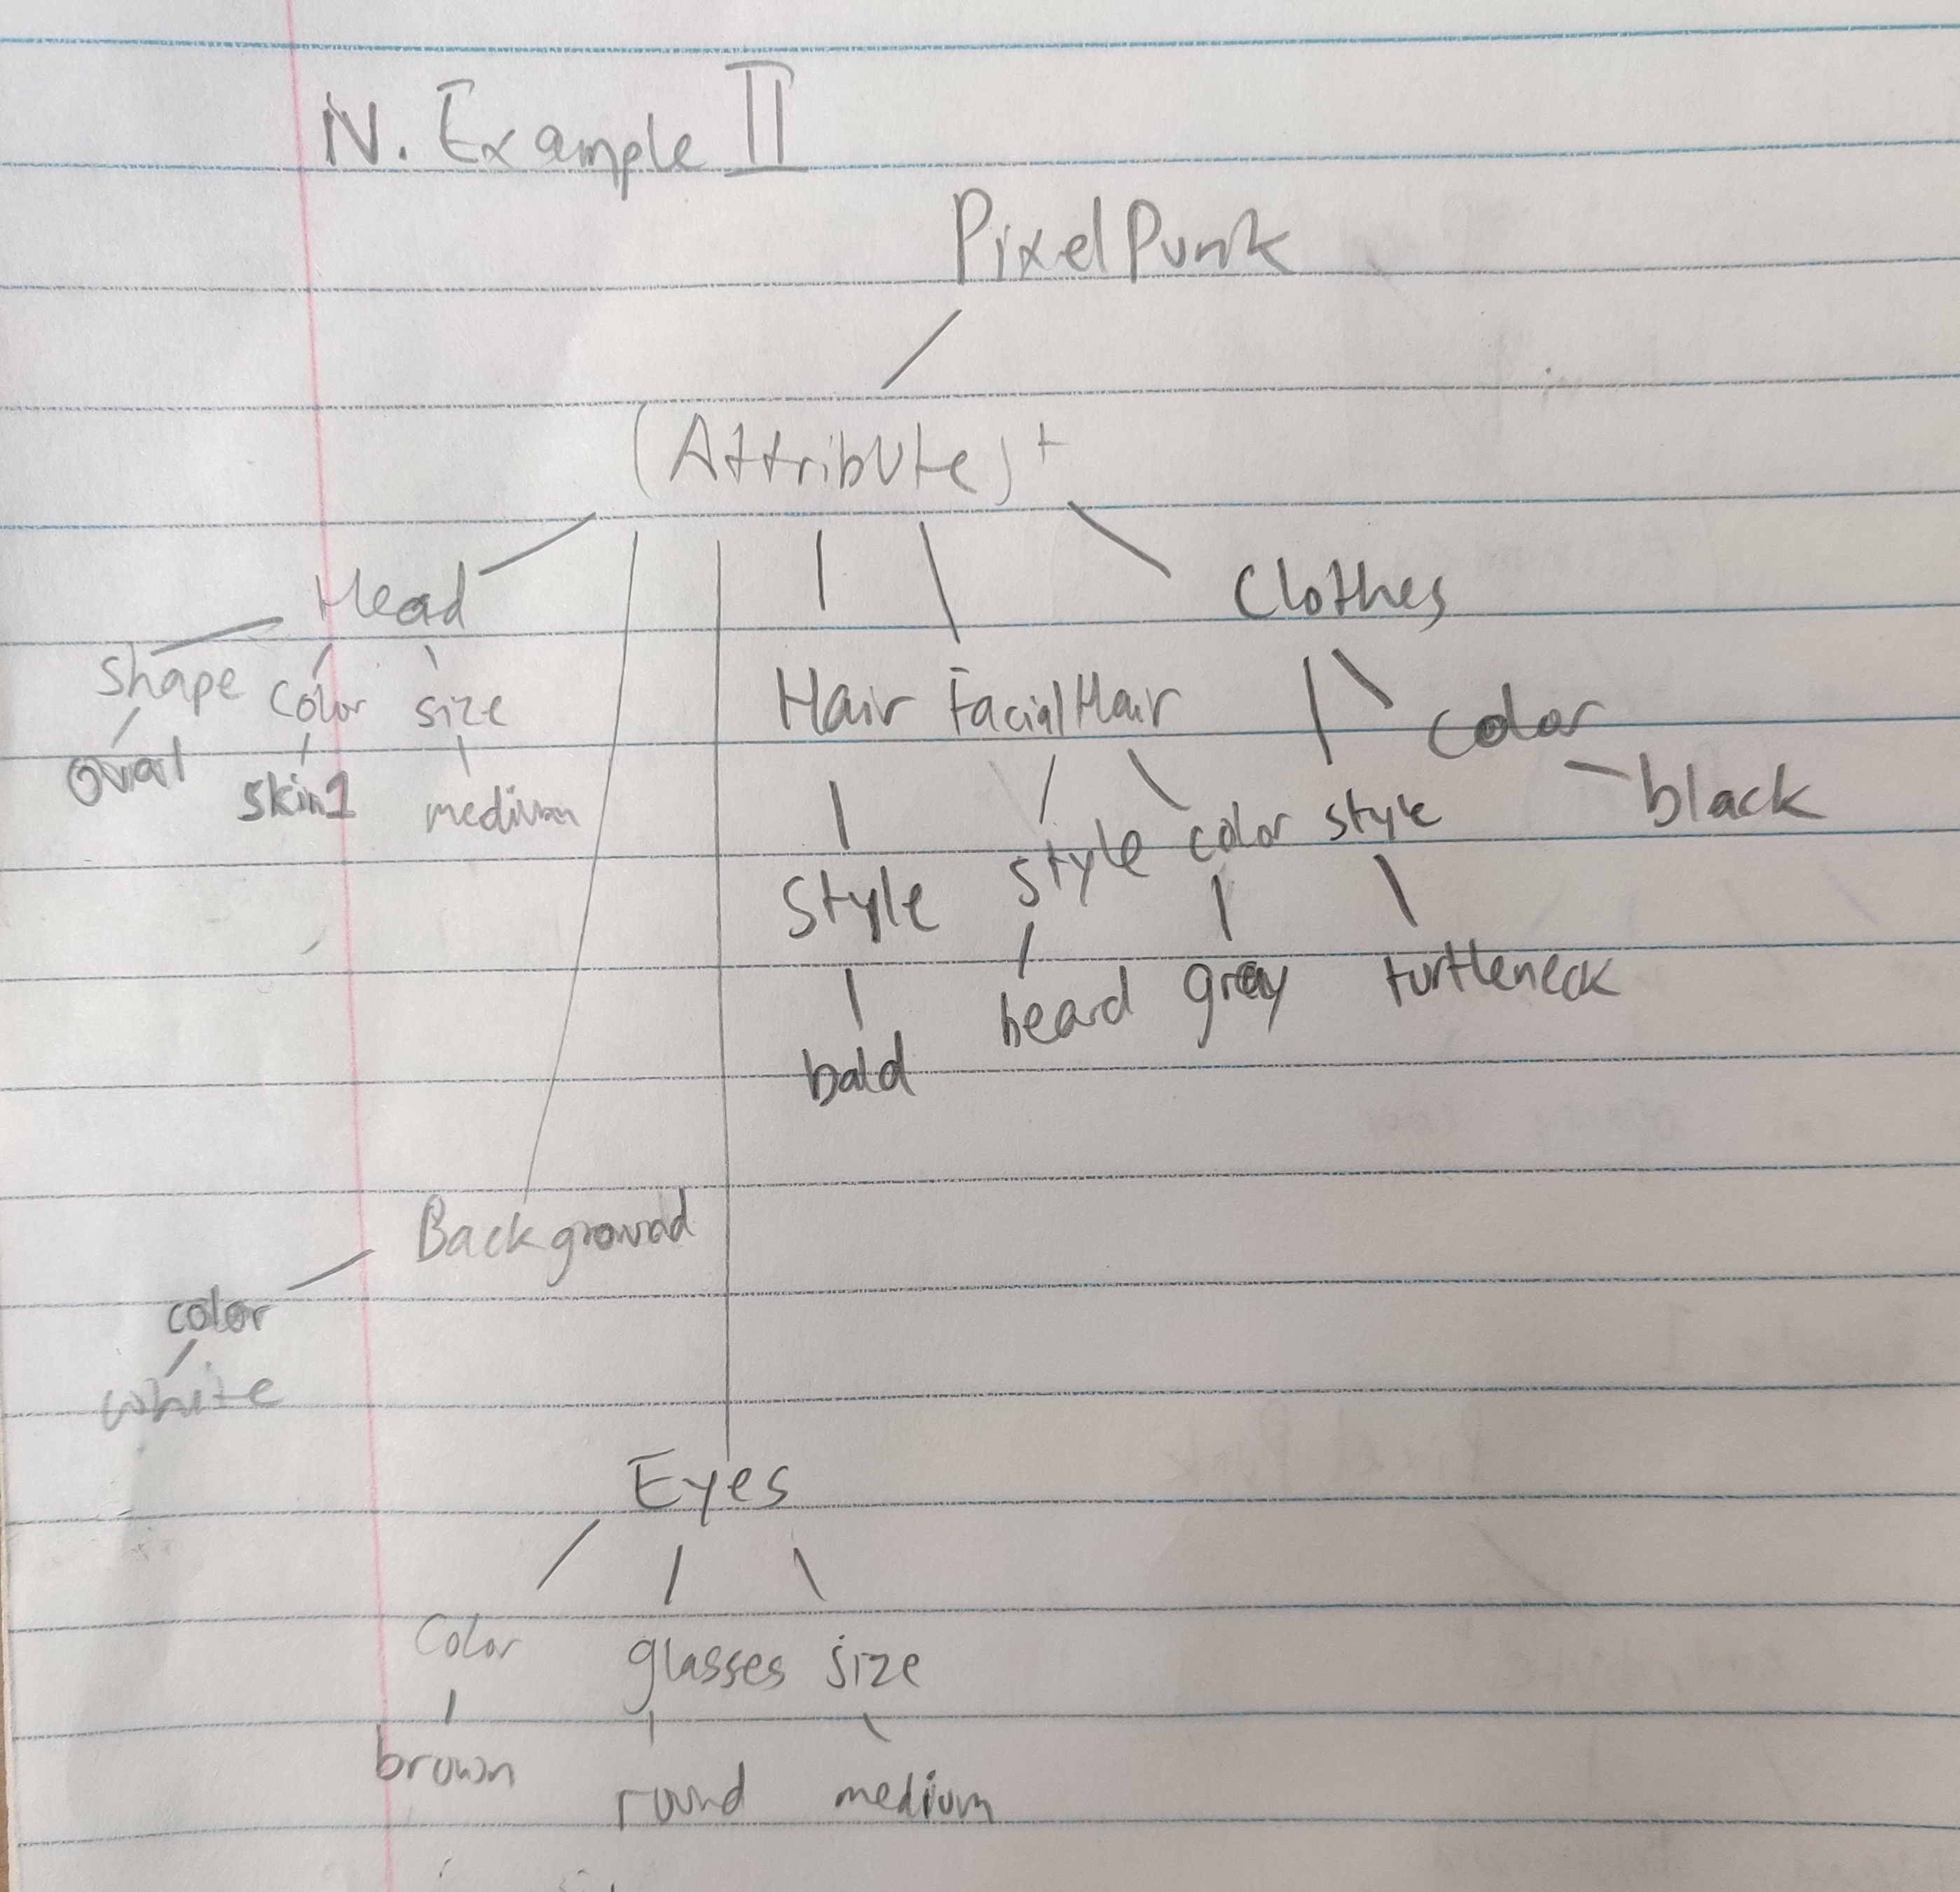
\includegraphics[width=0.75\textwidth]{images/example2.jpg}
    \end{center}
    \begin{center}
    	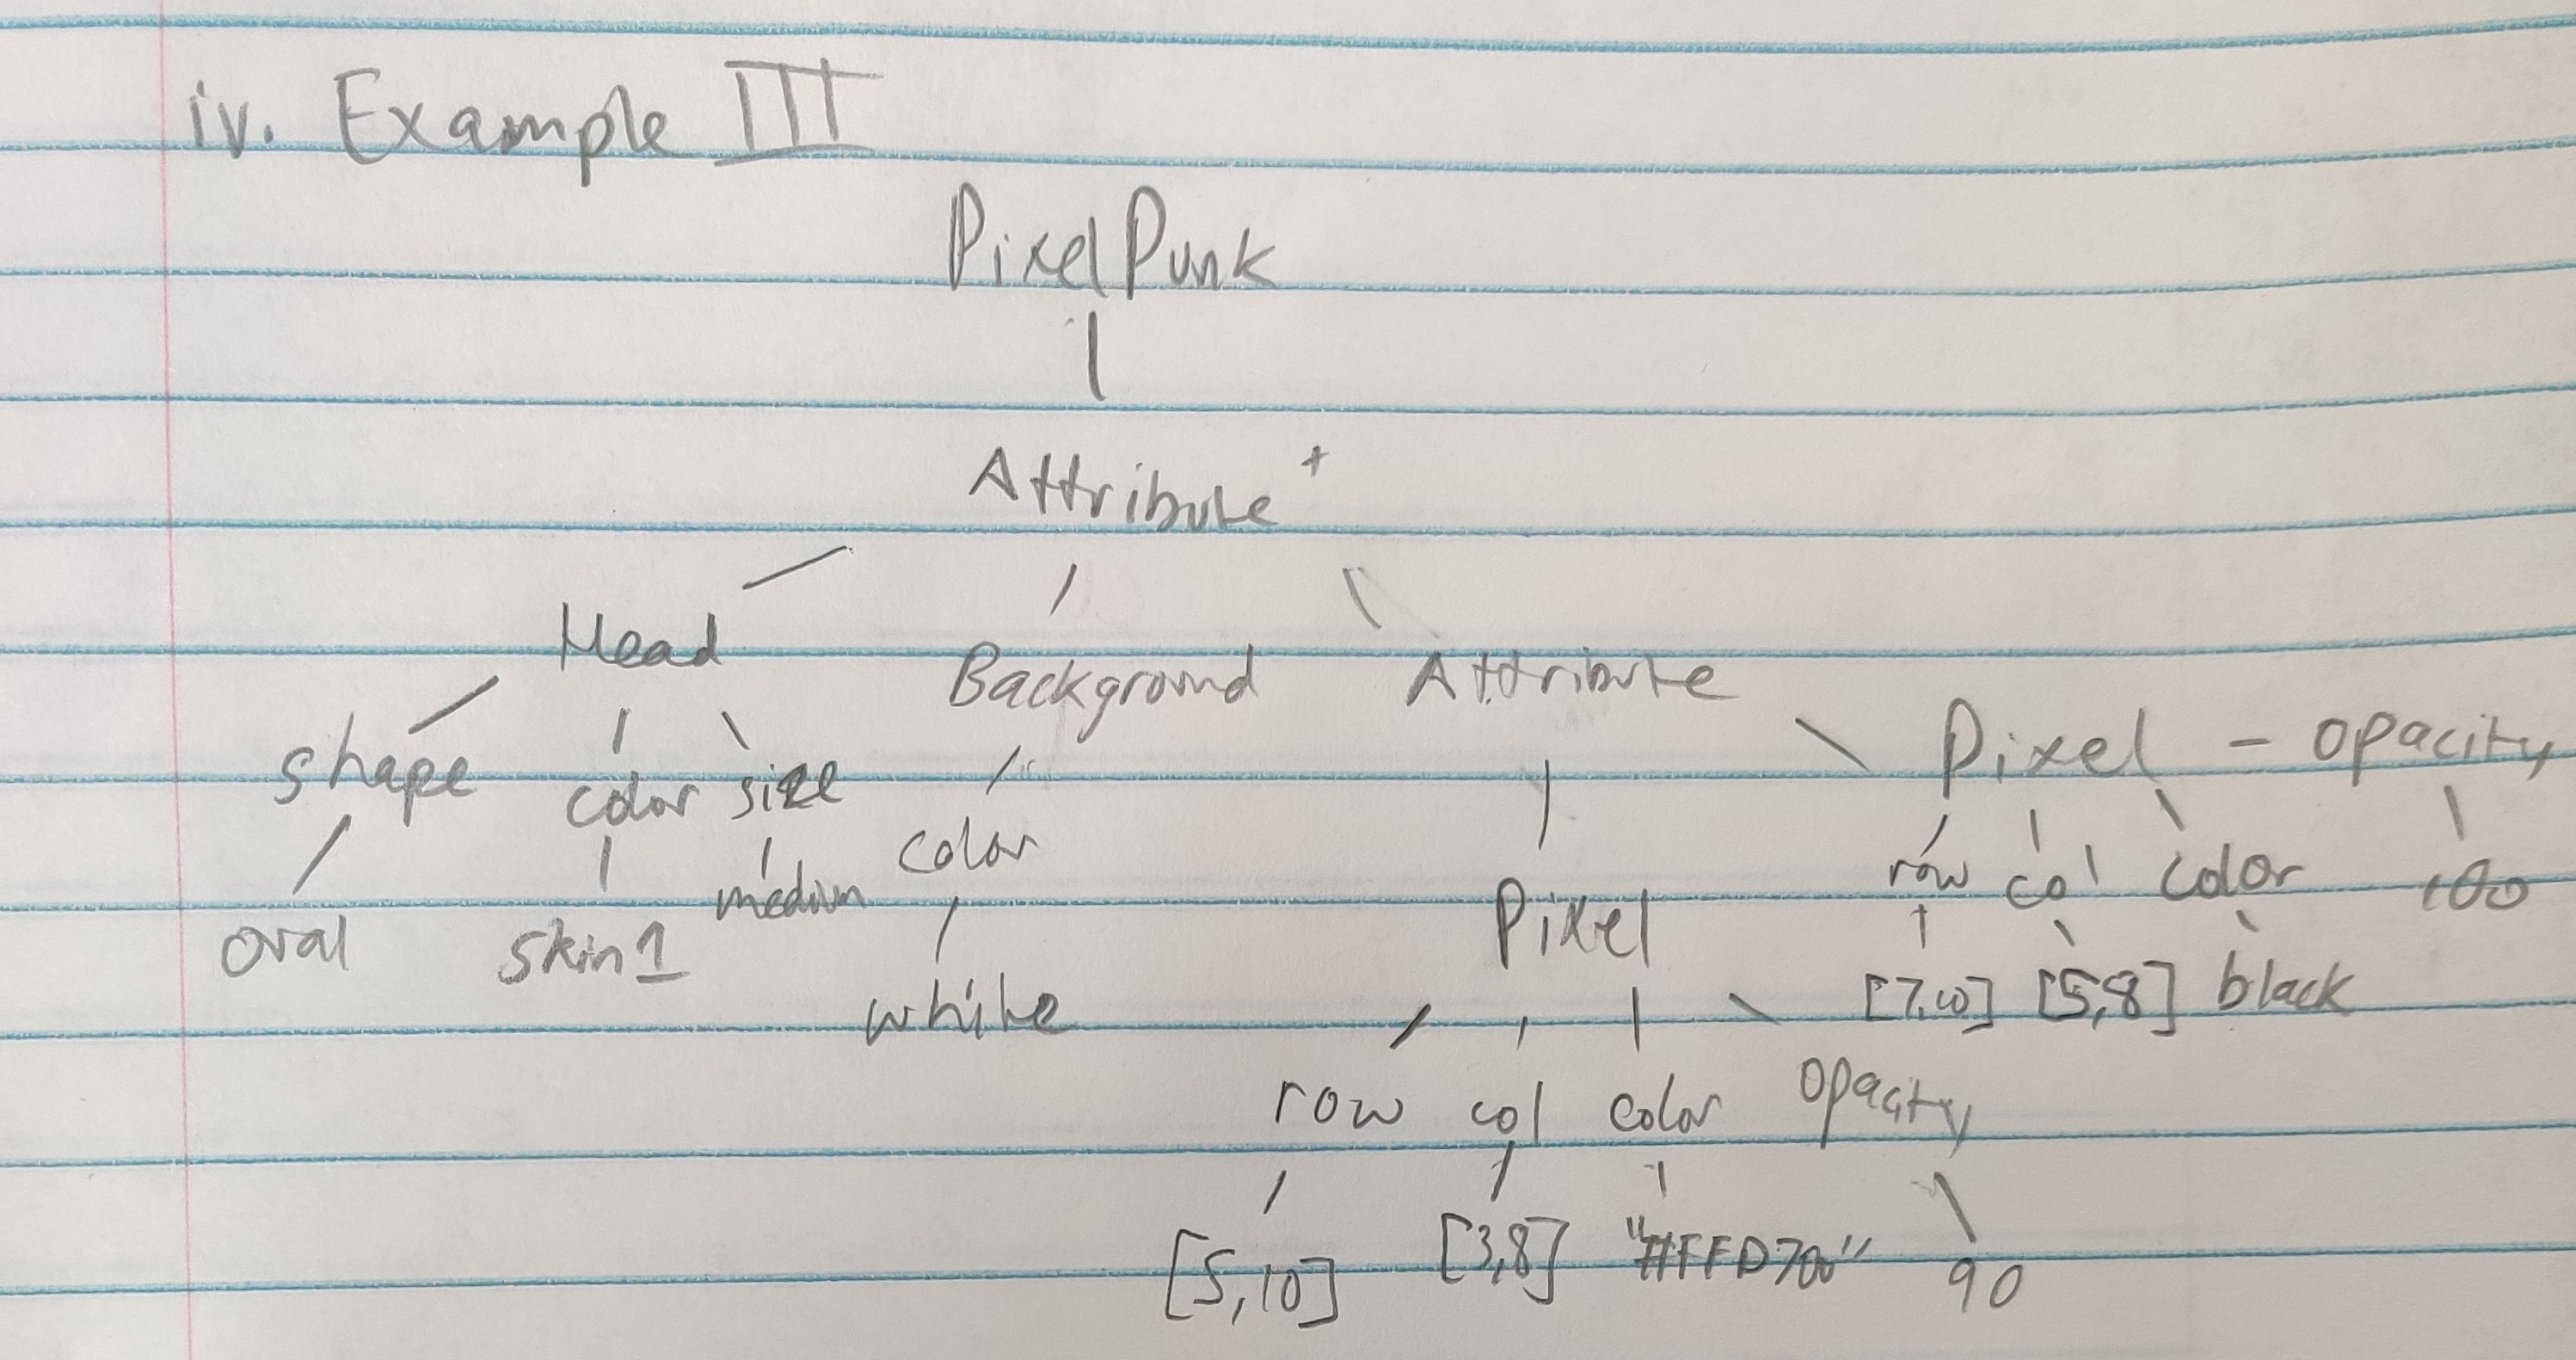
\includegraphics[width=0.75\textwidth]{images/example3.jpg}
    \end{center}
    
    \item
        \begin{enumerate}
            \item Programs in this language do not read any input.
            \item The effect of evaluating a program is a 24x24 pixel grid in a svg file that is a pixel art profile picture.
            \item A post-order traversal of the AST would yield the described effect because we're essentially combining pixels into attributes and then combining attributes into PixelPunks.
            
            Here is how the evaluation would work for example program 1:
            
            Start by evaluating pixels. More specifically, modify the specified pixels by setting the right color and opacity.
            \begin{center}
    	        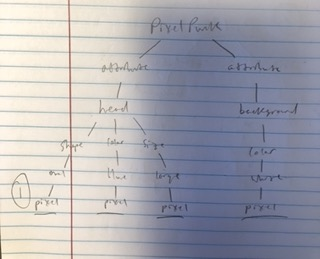
\includegraphics[width=0.75\textwidth]{images/astTraversal1.jpeg}
            \end{center}
            
            Next, combine pixels into attributes.
            \begin{center}
            	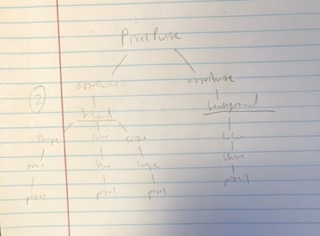
\includegraphics[width=0.75\textwidth]{images/astTraversal2.jpeg}
            \end{center}
            
            Finally, combine attributes into a PixelPunk.
            \begin{center}
            	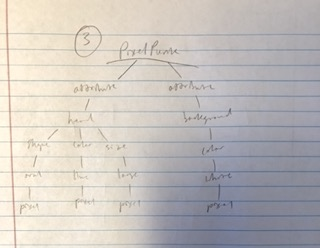
\includegraphics[width=0.75\textwidth]{images/astTraversal3.jpeg}
            \end{center}
            
            Ultimately, our evaluator will process the AST and output the PixelPunk grid as svg code into a PixelPunk.svg file, which can be opened easily in a browser such as Chrome for your viewing pleasure. 
        \end{enumerate}
    \end{enumerate}

% DO NOT DELETE ANYTHING BELOW THIS LINE
\end{document}
